\chapter{Modelling}
In this chapter the framework is built to represent the underactuated spacecraft problem. First the attitude control of a satellite is described, including the kinematics and dynamics. Then the orbit and environment are described, including the dominant disturbances acting on a satellite in low earth orbit. Finally the reaction wheel dynamics are described, with relevant fault mechanisms investigated.

\par\vspace{1cm}
A note on notation in this thesis:
\begin{itemize}
    \item 3D Vectors are denoted by bold lowercase letters, e.g.\ $\vec{x}$.
    \item Matrices are denoted by bold uppercase letters, e.g.\ $\mathbf{A}$.
    \item Scalars are denoted by lowercase letters, e.g.\ $a$.
    \item 4D vectors/matricies are denoted by bold lowercase/uppercase letters with a bar, e.g.\ $\vec{\bar{q}}$ $\vec{\bar{Q}}$.
\end{itemize}


\section{Attitude Control of a Satellite}
\subsection{Reference Frames and Attitude Representations}
Since the goal is to control the attitude of a satellite, an appropriate representation should be used. Any orientation can be representead as a rotation from one frame to another. Typical reference frames would be earth centered inertial (ECI), earth-centered-earth-fixed (ECEF), orbit or body-fixed. The satellite's orientation can be represented intuitively using euler angles yaw $\psi$, pitch $\theta$ and roll $\phi$, also known as the aerospace sequence. While these are intuitive, they suffer from singularities when trying to represent certain rotations. The direction cosine matrix (DCM) is the most fundamental representation of a rotation, since it is the rotation operator itself rather than a parameterization of it — it acts directly on a vector and is free of the singularities and sign ambiguities present in other representations. It can be used to transform a vector from frame A to B using the following relation 
\begin{equation}
    \vec{v}_B = \mathbf{C}^{BA}\vec{v}_A
\end{equation}

where $\mathbf{C}^{BA} \in \mathbb{R}^{3 \times 3}$ is the DCM from frame A to B and is made up of the orthonormal basis vectors of frame B expressed in frame A: $\mathbf{C}^{BA} = \begin{bmatrix} \hat{a}_1^B & \hat{a}_2^B & \hat{a}_3^B\end{bmatrix}$.

This matrix can be described by the euler 3-2-1 rotation sequence as:

\begin{align}
    % \begin{split}
    \mathbf{C}^{AB} &= \begin{bmatrix}
        c_{11} & c_{12} & c_{13} \\
        c_{21} & c_{22} & c_{23} \\
        c_{31} & c_{32} & c_{33}
    \end{bmatrix} \\
    &= \begin{bmatrix}
        C \psi C \theta &  S\psi C \theta & - S \theta \\
        - S \psi C \phi + C \psi S \theta S \phi & C \psi C \phi +  S\psi S \theta S \phi & C \theta S \phi \\
        C \psi S \theta C \phi + S \psi S \phi & S \psi S \theta C \phi - C \psi S \phi & C \theta C \phi
    \end{bmatrix} 
\end{align}

The given problem requires computing attitude kinematics over time, and while DCMs can be used for this purpose, it is cumbersome requiring computationaly expensive trignometric functions. Instead quaternions, $\vec{\bar{q}} = \begin{bmatrix}q_{x} \ q_{y} \ q_{z} \ q_{w}\end{bmatrix}^T$, are used to represent the kinematic differential equations. Quaternions represent a 4 dimensional extension of complex numbers. In order to represent rotations we limit ourselves to the unit quaternion which satisfies $q_{x}^2 + q_{y}^2 + q_{z}^2 + q_{w}^2 = 1$.

Any sequence of rotations can be represented as a single rotation by angle $\Phi$ about some vector $\vec{e}$. The rotation quaternion can be represented in these terms as:

% \begin{align}
$$
    q_{x}=e_{x}\sin(\Phi), \
    q_{y}=e_{y}\sin(\Phi), \
    q_{z}=e_{z}\sin(\Phi), \
    q_{w}=cos(\Phi)
$$
% \end{align}

The quaternion can be used to compute the DCM as follows:

\begin{align}
    \mathbf{C} = \begin{bmatrix}
        q_{x}^2 -q_{y}^2 - q_{z}^2 + q_{w}^2 & 2(q_{x}q_{y} - q_{z}q_{w}) & 2(q_{x}q_{z} + q_{y}q_{w}) \\
        2(q_{x}q_{y} + q_{z}q_{w}) & -q_{x}^2 + q_{y}^2 - q_{z}^2 + q_{w}^2 & 2(q_{y}q_{z} - q_{x}q_{w}) \\
        2(q_{x}q_{z} - q_{y}q_{w}) & 2(q_{y}q_{z} + q_{x}q_{w}) & -q_{x}^2 - q_{y}^2 + q_{z}^2 + q_{w}^2
    \end{bmatrix}
\end{align}

Quaternion multiplication is defined according to the hamiltonian (right-handed) convention as follows:
% \begin{align}

% \end{align}

\subsubsection{Rotation Operators}
There are a 2 ways of using rotation operators, either active or passive. An active rotation rotates a vector in a fixed frame, while a passive rotation rotates the frame itself. The active rotation is the conjugate of the passive rotation $\vec{\bar{q}}_{active} = \vec{\bar{q}}^{*}_{passive}$. Quaternion multiplication 

In this thesis the passive rotation convention is used.

\subsection{Attitude Kinematics}
To describe the kinematics, the inertial angular velocity of the spacecraft $\vec{\omega} = \begin{bmatrix}\omega_1 \ \omega_2 \ \omega_3 \end{bmatrix}$ now can be expressed in terms of quaternions in the following manner:


$$\begin{bmatrix} \omega_1 \\ \omega_2 \\ \omega_3 \\ 0 \end{bmatrix} = 2 
\begin{bmatrix} q_{w} & q_{z} & -q_{y} & -q_{x} 
            \\ -q_{z} & -q_{w} & q_{x} & -q_{y} 
            \\ q_{y} & -q_{x} & q_{w} & -q_{z}
            \\  q_{x} & q_{y} & q_{z} & q_{w}
\end{bmatrix} 
\begin{bmatrix} \dot{q}_{x} \\ \dot{q}_{y} \\ \dot{q}_{z} \\ \dot{q}_{w} \end{bmatrix}$$

and can be rearranged to form

\begin{align}
    \vec{\dot{\bar{q}}}
=\frac{1}{2}
\begin{bmatrix}
q_{w} & -q_{z} & q_{y} \\ 
q_{z} & q_{w} & -q_{x} \\ 
-q_{y} & q_{x} & q_{w} \\ 
-q_{x} & -q_{y} & -q_{z} \\
\end{bmatrix} \begin{bmatrix}\omega_1 \\ \omega_2 \\ \omega_3 \\ 0 \end{bmatrix}
\end{align}

Since it is required to determine the attitude error for the controller, another useful relation is the quaternion error. The error quaternion can be calculated as:

\begin{align}
    \vec{\bar{q}}_{e} &=  \vec{\bar{q}} \otimes  \vec{\bar{q}}_{d}^{-1} \\
    &= \begin{bmatrix}
        q_{dw} & q_{dx} & q_{dy} & q_{dz} \\
        q_{dx} & -q_{dw} & -q_{dz} & q_{dy} \\
        q_{dy} & q_{dz} & -q_{dw} & -q_{dx} \\
        q_{dz} & -q_{dy} & q_{dx} & -q_{dw} \\
    \end{bmatrix}
    \begin{bmatrix}
        q_{w} \\
        q_{x} \\
        q_{y} \\
        q_{z} \\
    \end{bmatrix}
    &= \vec{\bar{q}} \otimes  \vec{\bar{q}}_{d}^{-1}
\end{align}

the 

\subsubsection{Underactuated Case}
For the underactuated case, the error 


\subsection{Attitude Dynamics}

For the purposes of this thesis as a rigid body. The angular acceleration $\vec{\dot{\omega}}_{BI}$ of a rigid body with mass moment of inertia $\vec{J}$ can be modelled using the Newton-Euler equation:

\begin{equation}
\vec{J}\vec{\dot{\omega}} = \sum{\vec{T_{ext}}} -\vec{H}\times\vec{\omega}
\end{equation}
where $J$ is the satellite's mass moment of inertia, $\vec{T_{ext}}$ is any external torque applied and $\vec{h}$ is the total angular momentum of the satellite. Since we are focusing on reaction wheel control system

\begin{equation}
\mathbf{J}\vec{\dot{\omega}} = \mathbf{T}_d -\vec{\omega}^\times(\mathbf{J}\vec{\omega}-\vec{h}_w)-\dot{\vec{h}}_w - \vec{T}_{mag}
\end{equation}

where $\vec{T}_d$ represents the external disturbances applied, $\vec{h}_w$ represents the total reaction wheels angular momentum vector, and $\vec{T}_{mag}$ represents the magnetorquer applied torque. $\vec{\omega}^\times$ represents the skew symmetric matrix of the body angular velocity vector.

\section{Orbit and Environment}
A common orbit used for observation satellites is a sun-synchronous low earth orbit (LEO). This orbit allows the satellite to pass over the same part of the earth at the same local solar time. This is useful for imaging and observation as the lighting conditions will be similar for each pass. A typical altitude for a sun-synchronous LEO is between 400 and 800 km. 

Disturbance torques acting on a satellite in LEO are:
\begin{itemize}
    \item Aerodynamic drag torque
    \item Gravity gradient torque
    \item Solar radiation pressure torque
    \item Magnetic Dipole torque
\end{itemize} 

\subsection{Aerodynamic Torque}
Aerodynamic drag forces arise from the interaction of the satellite with the residual atmosphere present in LEO. Although the drag force is complex and time-varying due to atmospheric density fluctuations, it can be approximated under simplifying assumptions \cite{auretDesignAerodynamicAttitude2011}. For a near-circular orbit, the angle $x_{o,east}$ between the co-rotating atmosphere and the orbital path is given by

\begin{equation}
    x_{o,east} = \begin{cases}
        \pi - \arctan\!\left(\dfrac{d\lambda/dt}{d\phi/dt}\right) & \text{for } \dfrac{d\phi}{dt} < 0 \\[8pt]
        \dfrac{\pi}{2} & \text{for } \dfrac{d\phi}{dt} = 0 \\[8pt]
        -\arctan\!\left(\dfrac{d\lambda/dt}{d\phi/dt}\right) & \text{for } \dfrac{d\phi}{dt} > 0
    \end{cases}
\end{equation}

where $\lambda$ is the satellite latitude and $\phi$ is the longitude. The local atmospheric velocity vector expressed in the satellite body coordinate (SBC) frame is then

\begin{equation}
    \vec{v}^B_A = \mathbf{C}_{BO}
    \begin{bmatrix}
        -\|\vec{v}_o\| + \omega_E \|\vec{R}\| \cos(\lambda)\cos(x_{o,east}) \\
        -\omega_E \|\vec{R}\| \cos(\lambda)\sin(x_{o,east}) \\
        0
    \end{bmatrix}
\end{equation}

where $\|\vec{v}_o\|$ is the orbital speed, $\omega_E$ is the Earth's rotation rate, and $\vec{R}$ is the orbital radius. The atmospheric density $\rho$ required to evaluate the drag torque can be estimated with an exponential model

\begin{equation}
    \rho = \rho_0 \exp\!\left(-\frac{h - h_0}{H}\right)
\end{equation}

where $h$ is the orbit altitude, $h_0$ is a reference base altitude, $H$ is the atmospheric scale height, and $\rho_0$ is the nominal atmospheric density at $h_0$. The aerodynamic disturbance torque contribution of a given satellite surface is then \cite{auretDesignAerodynamicAttitude2011}

\begin{equation}
    \vec{\tau}_{\text{aero}} = \rho \|\vec{v}^B_A\|^2 A_p \left[\sigma_t\left(\vec{r}_{m/p} \times \bar{\vec{v}}^B_A\right) + \left(\sigma_n \frac{v_b}{\|\vec{v}^B_A\|} + (2 - \sigma_n - \sigma_t)\cos\alpha\right)\!\left(\vec{r}_{m/p} \times \bar{\vec{n}}\right)\right]
    \label{eq:aero_torque}
\end{equation}

where $\cos\alpha = \bar{\vec{v}}^B_A \cdot \bar{\vec{n}}$ is the cosine of the incidence angle of the atmospheric velocity on the surface, $\bar{\vec{v}}^B_A$ is the unit atmospheric velocity vector, $\bar{\vec{n}}$ is the inward-pointing unit normal of the surface, $\vec{r}_{m/p}$ is the vector from the centre of mass to the centre of pressure, $A_p = \mathcal{H}\{\cos\alpha\}\cos\alpha\, A_{\text{surface}}$ is the effective projected area (with $\mathcal{H}\{\cdot\}$ the Heaviside function), and $\sigma_n$, $\sigma_t$ are the normal and tangential accommodation coefficients respectively. The total aerodynamic torque is obtained by summing \eqref{eq:aero_torque} over all exposed surfaces.

\subsection{Gravity Gradient Torque}
The gravity gradient disturbance torque \cite{wertz1999space} on a satellite is caused by the gravitational differential across a body orbiting near another large body (Earth). This force is inversely proportional to the magnitude of the orbital radius $R_E$ cubed and is thus only significant in LEO.

The gravity gradient torque can be determined by \cite{wertz1999space}:
\begin{equation}
    \vec{\tau}_{GG} = \frac{3\mu}{{R_E}^3} \vec{u}_e \times (\mathbf{J_B}\vec{u}_e)
\end{equation}

where $\mu = 398600.5 km^3/s^2$ is the gravitational constant of Earth, $\vec{u}_e = \mathbf{C}^{OB} \begin{bmatrix}0 \ 0 \ 1\end{bmatrix}^T$ is the unit vector towards nadir in satellite body coordinates and $J$ is the satellite's moment of inertia tensor.


\subsection{Solar Radiation Pressure Torque}

\subsection{Magnetic Dipole Torque}
Satellites have a significant current running through their solar panels and wiring. The interaction between this current and the Earth's magnetic field produces a disturbance torque on the satellite. However with clever design this can be minimized. Solar panel manufacturers design their solar panels to mitigate this effect by using a balanced wiring layout. As such this torque is usually negligible and will be ignored in the analysis of the satellite's attitude dynamics. 

\section{Attitude Control}
\section{Reaction Wheels}

Reaction wheel dynamics can be modelled as a simple DC motor with a flywheel attached to the shaft. Sidi \cite{sidiAttitudeDynamicsKinematics1997} models the dynamics of the reaction wheel as follows:

\begin{figure}
    \centering
    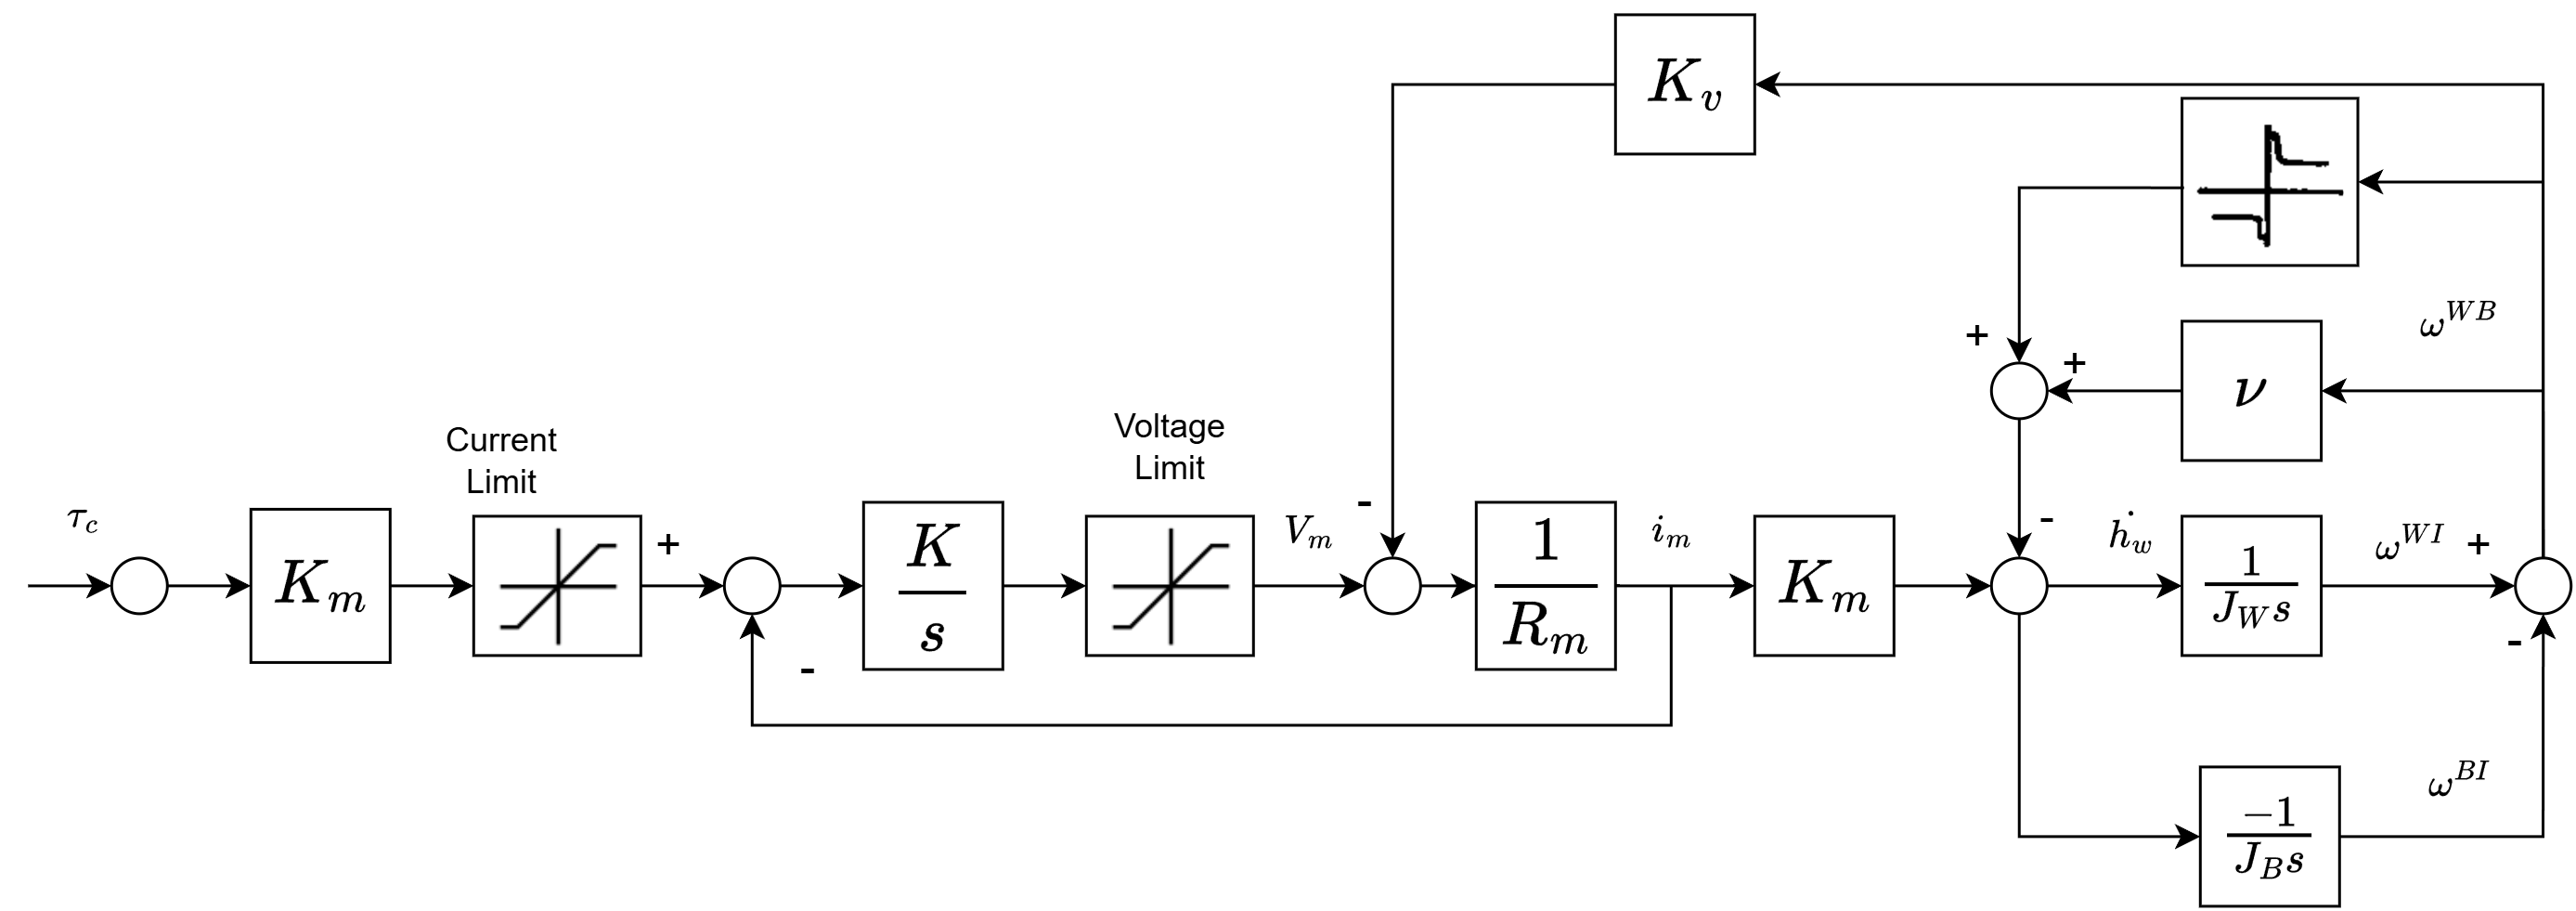
\includegraphics[width=1.0\linewidth]{chapter_3/Reaction_Wheel_Model.drawio.png}
    \caption{Reaction Wheel Dynamics Model \cite{sidiAttitudeDynamicsKinematics1997}}
    \label{fig:rw_dynamics}
\end{figure}

where $T_c$ is the commanded torque, $K_M$ is the motor torque constant, $K$ is the current-loop integrator gain, $V_M$ is the motor terminal voltage, $R_M$ is the motor winding resistance, $i_M$ is the motor armature current, $K_v$ is the back-EMF constant, $\dot{h}_w$ is the net torque delivered to the wheel, $I_W$ is the reaction wheel moment of inertia, $\omega_W$ is the resulting wheel angular velocity, $B$ is the wheel bearing viscous friction coefficient which is combined with the block describing the coloumb and dry friction to be fed back into the into the wheel torque, $\omega_{WB}$ is the wheel angular velocity relative to the spacecraft body (used to compute the friction torque), $I_B$ is the spacecraft body moment of inertia, and $\omega_B$ is the spacecraft body angular velocity, which combines with the wheel torque to give the net reaction torque on the body.

$K_M$, $K$ and $V_M$ are usually not supplied by the manufacturer of a COTS reaction wheel so control system designers typically use a simplified model. Typically a COTS reaction wheel is controlled by an internal PID controller which takes the error between the commanded and actual wheel speed and outputs a voltage to the motor. Since the response of the wheel is much faster than that of the spacecraft, the wheel torque can be considered to be applied instantaneously to the spacecraft. Thus, the internal motor dynamics can be neglected. Since the wheel is spinning at high speed relative to the satellite, the satellite's angular velocity can be neglected in the wheel dynamics. Thus the simplified reaction wheel dynamics can be modelled as:

\begin{figure}
    \centering
    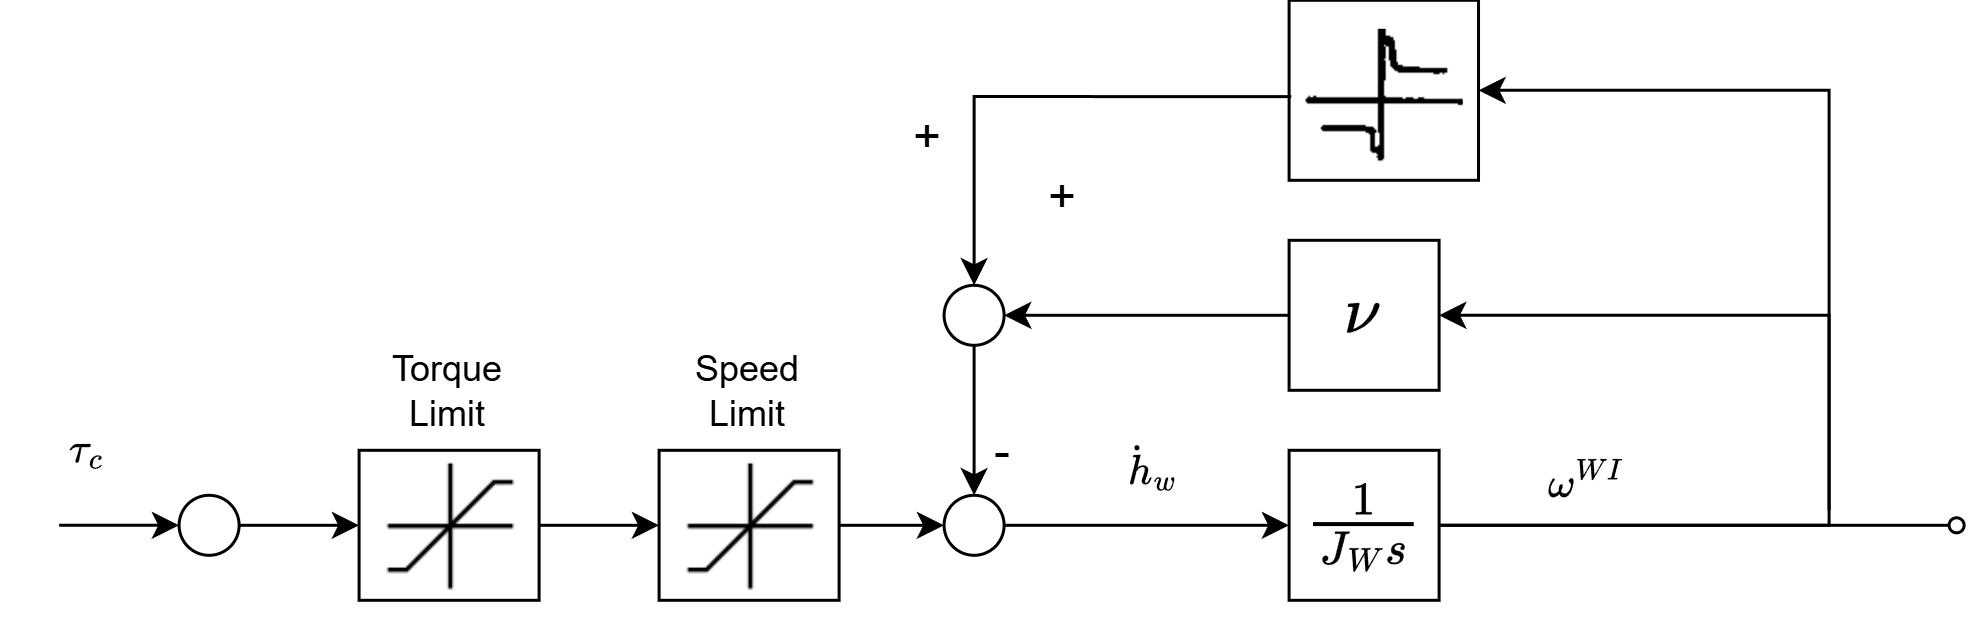
\includegraphics[width=1.0\linewidth]{chapter_3/Reaction_Wheel_Model_Simplified.drawio.png}
    \caption{Reaction Wheel Dynamics Model \cite{sidiAttitudeDynamicsKinematics1997}}
    \label{fig:rw_dynamics}
\end{figure}

\subsection{Reaction Wheel Faults}
Faults in reaction wheels can be broadly categorized as follows \cite{ZarouratiMohammad2023Daar}. Four representative fault types are defined according to how the wheel's speed characteristic deviates from its commanded value:

\begin{itemize}
    \item \textbf{Speed decrease:} the wheel speed remains proportional to, but scaled below, the desired value, producing a torque with high ripple. This is classified as a partial loss of effectiveness (PLOE) fault.
    \item \textbf{Deviation:} the wheel speed deviates from the desired value for some reason, producing a continuous bias torque. Since the actuator still generates a (non-zero) torque, this is classified as a hard-over failure with total loss of effectiveness (TLOE).
    \item \textbf{Stuck:} the wheel suddenly stops rotating following a step change, with bearing friction bringing the speed to zero over a characteristic time $T_z$.
    \item \textbf{Idle:} the wheel stops responding to commands altogether, and its speed remains frozen at whatever value it had at the instant the fault occurred.
\end{itemize}

Of these, only the stuck and idle faults produce no reaction torque whatsoever, and it is these two fault types that render the corresponding control axis underactuated, since all actuation authority on that axis is lost. The speed-decrease and deviation faults still produce some control torque and therefore do not by themselves create an underactuated configuration, although a speed-decrease fault can combine with a superimposed bias to form a compound loss-of-effectiveness-plus-bias fault. At the attitude control subsystem level, these actuator-level faults manifest as degraded pointing accuracy, reduced stability margins, and, for the remaining healthy wheels compensating for the fault, increased power consumption -- ultimately degrading image resolution and manoeuvrability and potentially leading to mission failure.

\section{Magnetics}
Reaction wheels, and other momentum based control methods, have the disadvantage, when compared to other control methods, that they build up momentum over time due to external disturbance torqures leading to actuator saturation. Thus to in order to manage this momentum, the earth's magnetic field can be utilized for generating small torques in LEO. The earth's magnetic field can be approximated as a dipole field \cite{sidiAttitudeDynamicsKinematics1997}. The magnetic field strength at a distance r from the center of the earth can be calculated using the following equation:

\begin{equation}
    \begin{bmatrix}
        B_{x} \\
        B_{y} \\
        B_{z}
    \end{bmatrix} = \frac{m}{r^3} \begin{bmatrix}
        cos(\alpha - \eta_m)sin(\xi_m) \\
        cos(\xi_m) \\
        -2sin(\alpha - \eta_m)sin(\xi_m)
    \end{bmatrix}
\end{equation}

where $\alpha$ is the phase angle measured from the ascending node of the orbit relative to the earth's equator $\eta_m$, $\xi_m$ and $m$ is the magnetic moment of the earth. \cite{sidiAttitudeDynamicsKinematics1997} The magnetic field can be used for attitude control by using magnetorquers which generate a torque by interacting with the earth's magnetic field. The torque generated by a magnetorquer can be calculated using the following equation:

\begin{equation}
    \vec{T_m} = \vec{m} \times \vec{B}
\end{equation}

where $\vec{m}$ is the generated magnetic moment of the magnetorquer and $\vec{B}$ is the magnetic field strength at the satellite's location \cite{sidiAttitudeDynamicsKinematics1997}. Some important notes about magnetorquers are that they can only generate torque perpendicular to the magnetic field and that the magnetic field strength varies with the satellite's position in orbit. The magnetic field is strongest near the poles and weakest near the equator.  Therefore maneuvers will require careful management to ensure that the satellite can maintain control throughout its orbit after under fault condition.
